\subsection{DisGeNET} \label{subsec:DisGeNET}
\href{https://goo.gl/ewnpWZ}{DisGeNET} is a discovery platform designed to address questions concerning the genetic underpinning of human diseases by analysing GDAs \cite{DisGeNET2015}. It is maintained by the Integrative Biomedical Informatics (IBI) Group at the Universitat Pompeu Fabra in Barcelona, Spain. DisGeNET made a clear distinction between Gene--Disease Associations (GDAs) and Variant--Disease Associations (VDAs) even though VDA is a GDA subclass in their ontology (see Figure \ref{fig:disgenet_ontology}). Is not VDA a subclass of GDA like they explain in the ontology in their ontology in Figure \ref{fig:disgenet_ontology} ?

\subsubsection{Data sources}
DisGeNET is organised according to the type and level of curation (see Table \ref{tab:disgenet_data} and \href{https://goo.gl/ntXTjX}{DisGeNET statistics}. For simplicity and given that they consider GDA as a VDA parent in the DisGeNET ontology (see Figure \ref{fig:disgenet_ontology}), I will just consider VDAs as a subtype of GDAs that includes the \texttt{Genomic Alterations} class and their children: any SNP, deletion, insertion, indel, somatic SNV, substitution, sequence alteration, or tandem repeat.

\begin{table}[H]
    \centering
    \resizebox{\textwidth}{!}{
    \begin{tabular}{c|c|c|c|c|c}
    Source & Type & Genes & Diseases & GDAs & Description \\
    \hline
    
    \href{https://goo.gl/XtufGc}{UniProt} &
    C & 19027 & 6303 & 20722 &
    Curated protein functional information \cite{uniprot2017} \\
    
    \href{https://goo.gl/aTyMBE}{CTDh} &
    C & 7787 & 4929 & 25975 &
    Environmental chemicals, genes and diseases \cite{ctd2017} \\
    
    \href{https://goo.gl/89TfbR}{ClinVar} &
    C & 45546 & 5639 & 54888 &
    Genetic human variants and diseases \cite{clinvar2016} \\
    
    \href{https://goo.gl/KxxD8Y}{GWASC} &
    C & 15790 & 610 & 20719 &
    GWAS catalog \cite{gwasCatalog2017} \\
    
    \href{https://goo.gl/hUkKLf}{Orphanet} &
    C & 2661 & 6702 & 97547 &
    Rare disorders, genes, and orphan drugs \cite{orphanet2012} \\

    \href{https://goo.gl/mgFWK4}{PsyGeNET} &
    C & 1546 & 112 & 3757 &
    Psychiatric GDAs \cite{PsyGeNET2015} \\

    \href{https://goo.gl/gYHKF3}{HPO} &
    C & 2661 & 6702 & 97547 &
    Phenotypic vocabulary for human diseases \cite{humanPhenotypeOntology2014} \\
    
    \href{https://goo.gl/aTyMBE}{CTDr} &
    M & 22 & 13 & 31 &
    CTD for \textit{Rattus Norvergicus} \cite{ctd2017} \\
    
    \href{https://goo.gl/aTyMBE}{CTDm} &
    M & 22 & 13 & 31 &
    CTD for \textit{Mus Musculus} \cite{ctd2017} \\
    
    \href{https://goo.gl/zc52JW}{RGD} &
    M & 1076 & 629 & 4291 &
    Genomic and disease data of \textit{R Norvegicus} \cite{rgd2015} \\
    
    \href{https://goo.gl/iTNmRx}{MGD} &
    M & 1464 & 1323 & 1994 &
    Genomic and disease data of \textit{M Musculus} \cite{mgd2015} \\
    
    \href{https://goo.gl/y3keCN}{GAD} &
    L & 13318 & 3099 & 63063 &
    GWAS repository \cite{gad2004}. Retired on 09/01/2014 \\
    
    \href{https://goo.gl/szDDw6}{LHGDN} &
    L & 5941 & 1799 & 31468 &
    Semantic ML extraction of GDAs \cite{bundschus2008} \\
    
    \href{https://goo.gl/4Yau27}{BeFree}* &
    L & 35392 & 16274 & 453574 &
    Biomed Name-Entity Recogniser of GDAs \cite{bravo2015} \\
    
    Total &  & 100076 & 29539 & 696707 \\
    
    \end{tabular}}
    \caption{Original data sources used by DisGeNET v5.0 \cite{DisGeNET2015}, type (\textbf{C} for curated data sources, \textbf{M} for Animal model data sources, and \textbf{L} for literature evidence sources), number of genes or gene variants, number of diseases or phenotypes, number of Gene--Disease Associations (GDAs or VDAs) and brief description. Information obtained from
    \href{https://goo.gl/ntXTjX}{DisGeNET statistics} \label{tab:disgenet_data}}
\end{table}

*The document used to extract GDAs was defined by the following PubMed query:

\begin{center}
\emph{
\small{
("Psychiatry and Psychology Category"[Mesh] AND "genetics"[Subheading]) OR ("Diseases Category"[Mesh] AND "genetics"[Subheading]) AND (hasabstract[text] AND ("1980"[PDAT] : "2017"[PDAT]) AND "humans"[MeSH Terms] AND English[lang])
}
}
\end{center}


\subsubsection{Scores}
DisGeNet developed two different confidence scores\footnote{\url{https://goo.gl/aSJVAd}}: one for GDAs and another for VDAs that reflected the evidence across all data sources \cite{DisGeNET2015}. I simplified the formulas they used, also because they are wrong: VDA has just two literature sources (GAD and BeFree), it cannot be a sum of three sources. Both scores ranges form 0 to 1 and the explanation of the variables is in Table \ref{tab:equationDisgenet}:

$$ score_{gda} = C + M + \sum_{l=1}^3 L_l $$
$$ score_{vda} = C + \sum_{b=1}^2 B_b $$

Note that the values for $C$ are different between GDA and VDA, I have not described the different values for VDA. Where:

\[
C =
\left\{
 \begin{array}{l}
  0.6 \quad if \quad c > 2 \\
  0.4 \quad if \quad c = 2 \\
  0.2 \quad if \quad c = 1 \\
  0.0 \quad otherwise
 \end{array}
\right.
\]

\[
M =
\left\{
 \begin{array}{l}
  0.16 \quad if \quad m = 2 \\
  0.08 \quad if \quad m = 1 \\
  0.00 \quad otherwise
 \end{array}
\right.
\]

\[
L =
\left\{
 \begin{array}{l}
  0.08 \quad if \quad 100 \cdot R_l \geq 0.08 \\
  R_l \quad\quad if \quad 100 \cdot R_l < 0.08
 \end{array}
\right.
\]

\[
B =
\left\{
 \begin{array}{l}
  0.15 \quad if \quad 100 \cdot R_b \geq 0.15 \\
  R_b \quad\quad if \quad 100 \cdot R_b < 0.15
 \end{array}
\right.
\]

\begin{table}[H]
    \centering
    \resizebox{\textwidth}{!}{
    \begin{tabular}{c|c}
    Variable & Meaning \\
    \hline
    
    $c$ & Number of curated, GDA--suporting sources: Uniprot, CTD, Orphanet, PsyGeNet, HPO \\
    $m$ & Number of animal models supporting GDA: \textit{M musculus} and \textit{R Norvegicus} \\
    $R_l$ & Ratio between GDA supporting papers and total papers in the data source $l$ \\
    $l$ & Index for GDA literature sources: GAD, LHGDN, BeFree \\
    $R_b$ & Ratio between VDA supporting papers and total papers in the data source $b$ \\
    $b$ & Index for VDA literature sources: GAD, BeFree
    \end{tabular}}
    \caption{Meaning of the variables for the GDA score in DisGeNET \label{tab:equationDisgenet}}
\end{table}

Why do they define this arbitrary weights for the data types? Why do not they assess the variability of each data type to define clusters in an unsupervised method? Why they do not use \href{https://goo.gl/k6vEBj}{information or entropy gain methods} like Open Targets \cite{ferrero2017} to assign a weight of each data type?

\subsubsection{Disease Specificity Index (DSI)}
\label{subsubsec:dsi}
Genes can potentially be associated to multiple diseases (e.g. TNF) while genes are associated to a reduced number of diseases or even to a single disease \cite{DisGeNET2015}. The disease specificity index (DCI) is defined as:

$$ DSI = \frac{log_2(n) - log_2(N)}{log_2(1) - log_2(N)} $$

Why did they use this complicated formula? Why not the ratio of related diseases and total diseases? They could have taken the inverse to achieve the same ranking in a faster way. Demonstrated in a \href{https://goo.gl/zsegji}{Jupyter notebook} that their formula takes a 2-fold more time than mine.

$$ DSI_{david} = N / n $$

where $N$ is the total number of diseases in DisGeNET (20,370) and $n$ is the number of diseases associated to a given gene \cite{DisGeNET2015}. Example: TNF is associated to more than 1500 diseases, therefore $ DSI_{TNF} = 0.247 $

\subsubsection{Disease Pleiotropy Index (DPI)}
\begin{shadequote}
\textbf{Pleiotropy} (from Greek $\pi\delta\epsilon\iota\omega\nu$ or \emph{pleion}, "more", and $\theta\rho o\pi o\zeta$ or tropos, "way") occurs when one gene influences two or more seemingly unrelated phenotypic traits.
\end{shadequote}
The rationale is similar to the DSI in Section \ref{subsubsec:dsi}, but they considered the number of different MeSH disease classes of the diseases associated to a given gene and the total number of MeSH diseases classes in DisGeNET \cite{DisGeNET2015}. The disease pleiotropy index (DPI) is defined as:

$$ DPI = n_p / N_p $$

where $N_p$ is the total number of MeSH disease classes in DisGeNET (28) and $n_p$ is the number of different MeSH disease classes associated to a given gene \cite{DisGeNET2015}. Example: gene KCNT is associated to 5 different MeSH classes, even though it is also associated to 12 diseases, 2 disease groups, and 2 phenotypes. Therefore $DPI_{KCNT1} = 5/28 = 0.179$.

\subsubsection{Evidence Index}
The evidence index (EI) indicates the existence of contradictory results in publication from BeFree and PsyGeNET supporting GDAs. It is defined as:

$$EI = \frac{n_p}{N}$$

where $n_p$ is the number of publications that support a GDA whereas $N$ is the total number of publication with any evidence (positive or negative) regarding the same GDA.

\subsubsection{Disease Mapping}
DisGeNET used the Unified Medical Language System (UMLS) vocabulary. The repositories of GDAs use different disease vocabularies:
\begin{itemize}
    \item UniProt, CTD, and MGD use OMIM terms
    \item CTD, LHGDN, and RGD use MeSH
    \item CLINVAR and PsyGeNET use UMLS Concept Unique Identifiers (CUIs)
    \item GWAS Catalog uses EFO
    \item Orphanet identifiers were mapped using Orphanet cross--references
    \item GAD disease names were normalised with the UMLS Metathesaurus
\end{itemize}

\subsubsection{Gene Mapping}
For human genes, HGNC symbols (used for some entries in GAD), and Uniprot accession numbers (used by Uniprot) were converted to NCBI Entrez gene identifiers using an in--house dictionary that cross--references HGNC, Uniprot and NCBI-Gene information.

For mouse and rat genes, they used files \texttt{HOM\_MouseHumanSequence.rtp} and \texttt{RGD\_ORTHOLOGS.rtp} to map rat and mouse Entrez gene identifiers to human Entrez identifiers, respectively. These files are available somewhere else\footnote{\url{https://goo.gl/BJuBzY}}. Rat and mouse genes without human ortholog were discarded.

\subsubsection{Association Type Ontology}
For a seamless integration of GDAs data, they developed the DisGeNET association type ontology. All association types as found in the original source databases were formally structured from a parent \texttt{Gene Disease Association} class if there was a relationship between the gene/protein and the disease, and represented as ontological classes (see Figure \ref{fig:disgenet_ontology}).

\begin{figure}[H]
    \resizebox{\textwidth}{!}{
    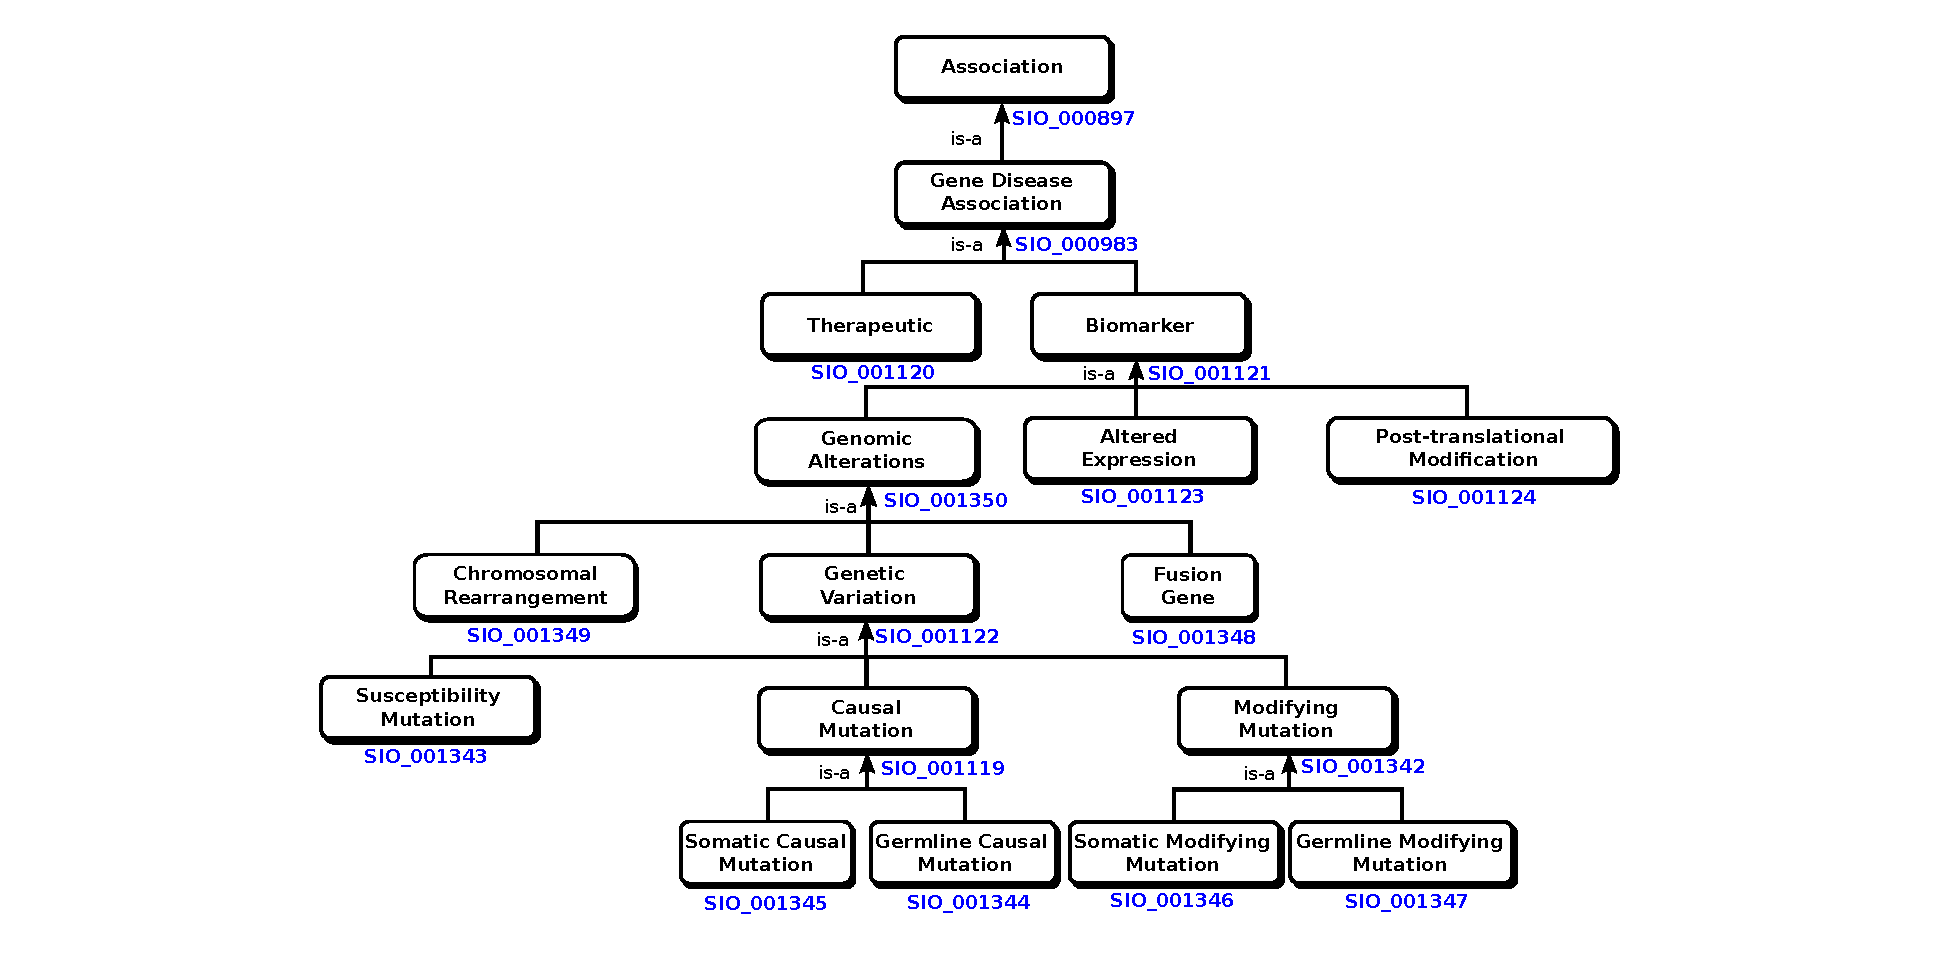
\includegraphics{pics/ontologyDisGeNET.pdf}}
    \caption{DisGeNET ontology \cite{DisGeNET2015}  \label{fig:disgenet_ontology}}
\end{figure}

Is not this similar to the already developed functional consequence score from Open Targets? It was obtained from \href{http://www.ontobee.org/ontology/SO?iri=http://purl.obolibrary.org/obo/SO_0001566}{OntoBee}

The labels from the original sources were mapped to DisGeNET Gene-Disease Ontology as detailed in Table \ref{tab:disgenet_ontology}.

\begin{table}[H]
    \centering
    \begin{tabular}{c|c}
    Association class & Original source label \\
    \hline
    
    \texttt{Altered Expression} & BeFree, LHGDN \\
    \texttt{Biomarker} & BeFree, HPO, LHGDN, MGD, PsyGeNET, RGD \\
    \texttt{Chromosomal Rearrangement} & Orphanet \\
    \texttt{Fusion Gene} & Orphanet \\
    \texttt{Genetic Variation} & BeFree, GAD, LHGDN, Orphanet, UniProt \\
    \texttt{Germline Causal Mutation} & Orphanet \\
    \texttt{Germline Modifying Mutation} & Orphanet \\
    \texttt{PostTranslational Modification} & BeFree, LHGDN \\
    \texttt{Somatic Causal Mutation} & Orphanet \\
    \texttt{Somatic Modifying Mutation} & Orphanet \\
    \texttt{Susceptibility Mutation} & ClinVar, Orphanet, RGD \\
    \texttt{Therapeutic} & CTD, RGD
    \end{tabular}
    \caption{Classification of the data sources into the \texttt{class nodes} in the DisGeNET ontology}
    \label{tab:disgenet_ontology}
\end{table}